\documentclass[conference]{IEEEtran}
\usepackage{url} 
\usepackage{cite}
\usepackage{amsmath,amssymb,amsfonts}
\usepackage{algorithmic}
\usepackage{graphicx}
\usepackage{textcomp}
\usepackage{xcolor}
\def\BibTeX{{\rm B\kern-.05em{\sc i\kern-.025em b}\kern-.08em
    T\kern-.1667em\lower.7ex\hbox{E}\kern-.125emX}}
\begin{document}

\title{Power laws in code repositories: A skeptical approach
  \thanks{ This paper has been supported in part by
    project DeepBio (TIN2017-85727-C4-2-P)}
} % Good title! 

\author{\IEEEauthorblockN{B. Ortiz}
  \IEEEauthorblockA{Geneura Team, ETSIIT and CITIC, University of Granada (Spain)\\
{\tt bortiz@ugr.es}}
\and
\IEEEauthorblockN{J. J. Merelo}
\IEEEauthorblockA{Geneura Team, ETSIIT and CITIC, University of Granada (Spain)\\
{\tt jmerelo@ugr.es}}\\
}

\maketitle

\begin{abstract}
  
  % Does self-organization imply power laws? Or a critical state? Self organization will take place even if a critical state has not been reached yet, right? - JJ
Software development as done using modern methodologies and source
control systems has been often established as an example of
self-organization, with code growing and evolving organically, through
activities that do not stem from centralized power, leader or
directives.  The main difficulty of these studies is that self
organization cannot be detected through direct observation, but
through measurements on the system, looking for features such as the
existence of powerlaws over some features (such as changes) and sizes.
Although published and proposed in many papers as such, power laws are
more elusive than they might seem at first sight, so in this paper we
present a statistically accurate set of tests that help us decide,
from the way repositories are changing, if they are really distributed
by a powerlaw, which could indicate us the existence of a state
reached via self-organization.

We revisit one of the most representative papers of these observations to reevaluate its results and compare them
with the current status of the repositories analyzed in it.

% Not clear what's the gist of this abstract. You can read it as 
% * We _know_ that code repositories self-organize
% * But we don't know how to detect self organization
% * So we have to find power laws
% * Some people have found them
% * But in many cases it's not statistically significant
% * We are going to propose a mathematical methodology to actually find power laws
% * And revisit our old paper and data to find out if it's really the case that there is a power law, or that we can't affirm that there is not one.


% Here we add the findings and conclusions

\end{abstract}

%\keywords{Complex systems, self-organizing systems, self-organized
%  criticality, power laws, artificial life,software development,software repositories}


%%%%%%%%%%%%%%%%%%%%%%%%%%%%%%%   INTRODUCTION   %%%%%%%%%%%%%%%%%%%%%%%%%%%%%%%
\section{Introduction}\label{introduction}

There are several steps in the study of self-organized systems  \cite{bak1988self}. One of
them is to study the existence of a power-law's distribution in the data
from our system. This property is intrinsically related to the scale-free behaviour
these systems exhibit, that is, systems where there is no single characteristic event size \cite{golyk20self}.
Understanding what distribution is producing our data gives us insights of
how confidently we are about claiming that our system is in a critical state, since this states
are usually correlated with the appearance of a power law \cite{newman2005power}. % cite needed -bart

Moreover, it is interesting to see if there is some kind of evolution in data. 
A change in the distribution that explain the data could be originated by a 
phase change, and phase change happend by passing a critical state. 

However, during this process, we have to justify every conclusion we get, not only 
by fitting our data, but by giving a proper statistical measure of the probability 
of our conclusions, that is, following an standarize mathematical method based on
hypothesis testing.% Clarify what you mean by "A distorted version of reality", saying clearly what you want: revisit claims for the existence of power laws, showing that in most cases they only seem a power law. - JJ

% * Why is self-organization in repositories important? What would it imply -JJ
% I 'm not sure about how to "attack" this question. - Bart

Following \cite{merelo2017self} approach, we are going to comprehend code repositories
by the interactions (events) made in them. Code repositories are one of the ways 
software is developped nowadays. Multiple platforms like gitlab or github 
offer the possibility of interact with the code making changes, adding and deleting 
lines. 
All these interactions are reflected in an archive by what we call commits. From it
we can obtain the data about how this code has been changed. 

But to really start to understand the behaviour of software development teams as
reflected by their activity in repositories, we should not
only try to fit a powerlaw in our data but making a statistically
accurate study to confirm how much evidence we have of this type of
behaviour. 

Most of the measures and estimations about powerlaws in code repositories are collected 
in studies like \cite{merelo2017self}, where some evidences of powerlaws are presented.
However, since there are better methods to study this data \cite{clauset2009power}, 
we are going to re-evalute all the results obtained, offering an alternative skeptic view
of the existence of power laws.

We have focused in this particular topic because of three reasons. 

First of all, there are no 
extensive analysis that addresses this question. We haven't found a comparative study 
that offers data-based statistical measures to check if the powerlaw assumptions hold.
So we are goint to fill this gap offering a complete statistically study about
the evidences of powerlaws behaviour in a variety of repositories.

Moreover, we are not going to evaluate just our evidences about the existence of a power law,
we are going to offer a short range of distributions that can generate similar results and could
easily be confounded by a powerlaw. This is an standard way to discover if our data is more likely
to be produced by other heavy-tailed distribution \cite{clauset2009power}, like the logNormal
or the truncated powerlaw. 

Finally, since we are able to access to multiple years' data, we also interested in study the
temporal evolution of the two previous analysis. Here our main objetive is to show how these measure could 
have changed (if they have at all). We should remember that repositories are evolving system
by definition, so they can experiment qualitative changes in his events distribution. Furthermore, even 
if they preserve their behaviour, they can still change some distribution's parameters.
To locate and analyze this changes could be translated in a deeper knowledge in the evolution 
of these system, specially in the presence of phase changes \cite{merelo2017self} or self-organized
critically (understood as a mechanism by which the system is regulating himself to stay in those 
parameters \cite{newman2005power}).


This way, we offer a test to analyze how much evidence there is for or
against our assumptions in every step, and a set of comparatives to identify some relevant temporal
changes, establishing a statiscally correct starting point to answer the question: Does software
development really follows a powerlaw? 

Next, we will explain our methodology followed by the results obtained,
closing with our conclusions. 

% --------------------------------------------------------


\section{State of the art}\label{soa}

The study of code repositories from the point of view of self-organized criticality has not followed a continuous line of investigation.

On the one hand, we find that self-organized criticality has been
Description of a wide variety of code repositories with a certain probability. These studies can be found in\cite{wu2007empirical,gorshenev2004punctuated}, but they are not the only ones of this kind. Tests on the possible self-organized criticality have also been sought in another type of repositories and projects, which are enumerable in size and purpose \cite{Merelo2016:repomining,merelo16:slash,merelo16:self,merelo2017self}.

In most of these studies, however, the evidences in favor of the existence of a power law are not accompanied by a significant statistical study. It is usual, as described in \cite{newman2005power} that the evidence leading to a suggestion of a power law in the distribution is visual. Once we have these tests, the study goes through the adjustment of a possible powerlaw \cite{merelo2017self,arafat2009commit}.

The general trend being the lack of statistical evidence that supports the hypothesis of the existence of a power law, the truth is that as described in \cite{newman2005power, clauset2009power} the most common method for making subsequent adjustments, Leas Square Medium \cite{merelo2017self,arafat2009commit,merelo16:self}, usually implies the existence of a greater error than the possible alternatives.

Currently, the general trend that started with the description of the power laws in self-organized systems has been slowed down. Instead, due to the existence of more objective evaluation methods, the results that were assumed until now are being re-evaluated.

Examples of this trend are papers such as \cite{Holme2019, Broido2019}, where the power laws in the networks and in the results will be reevaluated.

\cite{Jones2003}
\cite{voitalov2018scale}
\cite{Stumpf665}

\cite{merelo2017self,arafat2009commit,merelo16:self}

% below it is the soa of the previous paper

As far as we know, there has not been a continuing line of research on
self-organized criticality in software projects or, for that matter,
any other kind of collaborative work teams. The main reason might be
that researchers have thoroughly
proved that several big software repositories seem to be in a SOC state,
\cite{wu2007empirical,gorshenev2004punctuated}, although some
not-so-big and not-really-software repositories seem to be in that
state too \cite{Merelo2016:repomining,merelo16:slash,merelo16:self};
in these last papers suggest, that since these repositories have different characteristics in terms
of the number of users, age and type of information they hold implies that
self-organization, as it should be expected, is achieved with relative
ease and due to factors not related to the nature of the content being
developed, but the way the interaction is done itself. 

Indeed, this state of self-organized criticality
quantitatively proves what has been already established via
qualitative analysis, the fact that in many successful software
projects, developers self-organize \cite{Crowston2007564}, 
which is
the preferred way of working in distributed and volunteer
teams \cite{crowston2012free}. In fact, this way of organization
matches our own experience in development of open source projects such
as \cite{ae09,2016arXiv160101607M}, which are developed mainly by one
or a few coders, helped sporadically by other coders that find an
error and fix it or adapt the code to particular situations. 
In fact, this self-organization has also been observed in similar
projects such as Wikipedia \cite{10.1371/journal.pone.0017333}

A critical state might eventually emerge from self-organization
given the necessary conditions. However, there has been no work going further and
proving this even in the case that the team is carried out by a small team and
on repositories that are not devoted to software development. And this
critical state is key to carry the system to adaptive success, as
defined by \cite{benbya2006toward}, which presents 
the seven mechanisms that create complexity as initially enunciated for
biological systems and apply them to information system
development. 

One of these principles, the principle of {\em change rate}, which appears in the
way of observation-orientation-decision-action, is very explicit in
open source development, where you usually observe a repository or
project for a certain time, then find if there is something to fix or
the way you can adapt it to your particular circumstances, decide what
to do and how to do it, and, eventually, act on your fork, resulting in a
pull request to the original repository. These activities can
effectively be defined as social, so that teamwork in software
repositories is embedded in a kind of social
network. \cite{valverde2007self}
have proved how this network grows under the tension of top-down or
hierarchical rules and self-organization emerges from the bottom,
which makes software development teams a complex social system, indicating that the self-organized critical state would be much
more pervasive than initially thought. 

In this paper we will mine software repositories and take the measures
that would confirm they are in a self-organized critical
state. Eventually, our intention is to try and find the point when
phases change, although in this paper we will focus in studying the
existence of a self-organized criticality state in the repositories under study.
Next we
will present the methodology used to choose those repositories and
mine their information. 


% --------------------------------------------------------


\section{Methodology}
\label{sec:method}

\subsection{Data extraction}
We have chosen 16 repositories in different states of development,
which represent a wide array of languages and functionalities, from
web frameworks such as Django to Atom plugins, through one-of-a-kind
frameworks such as Docker. Normally a project includes several
different languages, and these languages are either
interpreted or compiled, either to machine code or to
bytecode. Repositories vary also in {\em professionalism}, from
a small Atom editor plugin for Perl6 to Docker, an open
platform for building and running isolated applications,
created and maintained by a fully professional community.

Repository mining was done during the months of January to March
2017, with the second sweep of the same repositories performed in
February 2019.

The way we look at changes in the repository was initially proposed by \cite{Merelo2016:repomining} and was also used in
\cite{merelo2017self}, where a deeper explanation can be found.

% We need to rewrite all of this.
This procedure is based on three main concepts:
\begin{itemize}
	\item The usage of a discrete timeline formed by the
	commits, with every commit counting as time=1. 
	\item Work with selected files in the repository, excluding 
	those related to images or style
	\item We take the largest value from the inserted and deleted lines of code.
\end{itemize}

Up to this point, there is nothing new. But is the way that we evaluate our results that differs from previous analysis.

\subsection{Hypothesis tests}

Once the information from the repositories has been extracted, we
proceed to analyze it in order to find clues about what kind of distribution is generating our data. 

With that particular objetive in mind, we change the methodology used
in \cite{merelo2017self} for several reasons.

First of all we want to offer a test that checks whether the observed data 
set actually follows a power-law, instead of only visualize the result. 
This kind of tests can vary based on differtent measured and techniques. The one we
are going to use is suggested in \cite{clauset2009power}, which consists in using a
goodness-of-fit hypothesis test via boostrapping procedure. 

Due to the use of boostrapping, this procedure is a time and resources consuming one.
We essentially  generate  multiple  data  sets  with our two main parameters $x_{min}$ 
and $\alpha$  and  then  we reinferr the model parameters. The outcome of the algorithm 
will result in a P-value, which, if is large enough, tell us that the difference
between our data and the powerlaw model we have generated is small and mostly attributed
to statisticall randomness. On the other hand, if P-value is close to 0, it is quite unlikely
that our model fits the data properly.
Following \cite{clauset2009power} we choose our treshold value in $p=0.01$, in addition
we are going to perfom this analysis with R package: PoweRlaw. A detailed description
of it and the hypothesis tests can be found in \cite{gillespie2015power}.

Up to this point, we have detected what datasets are unlikely to be fitted by a powerlaw
in any of its range. Notice, on the contrary case, that we are only assuming that
we can not discard that a powerlaw is generating the data.
However, as there is some probability of the appearance of this distribution in our data
we can study and analyze how its two main parameters may evolve between 2017 and 2019.

As it is unrealist to think that a powerlaw distribution will
fit all our data, our first step is to check what portion of the data
could be fitted with a powerlaw, or in other words, what is the minimal value 
(if there is one) from which the scaling relationship of the powerlaw begins
\footnote{This is a fair assumption since we are working with heavy-tailed distributions 
	and our main interest is the behaviour of the tail of our data.}. 
This value is usually noted by $x_{min}$ and is our first parameter.

Once we have the fisrt value, we proceed to estimate the scale of our powerlaw.
As it is shown in papers like \cite{newman2005power, clauset2009power},
least square method is a poor but widespreaded way to proceed when estimating the
scale parameter. Instead, we are going to use a direct method describe in
\cite{clauset2009power} and impletmented in \cite{alstott2014powerlaw} that use
the data values we have. This method is known to produce a very nice fit with
less error than the others mentioned above.

Up to this point we have revisited our way of analyze powerlaw fitting and
the estimation of our parameters. However, there is a more deep question unanswered:
does our data really follow (in a statiscally relevant way) a powerlaw?
This kind of answers were lacking in \cite{merelo2017self} and they are relevant
independently our first test's results, since they usually offer an unbiased look of the data . 

Taking into account that our main question is wether a powerlaw is the best 
description of our data, we choose to apply a comparative test that could 
evaluate if there are any alternative distribution that could have generated
our data with greater likelihood than a powerlaw. That is the main reason why
we choose to use a loglikehood ratio test implemented in \cite{alstott2014powerlaw}.
There are two algorithm's outcomes. First we have the loglikelihood ratio between the 
two  candidate  distributions. The sign of this quantity will point out which
distribution is more likely to be producing out data. After it, we calculate the signification 
of this ratio, a P-value. Following \cite{alstott2014powerlaw} indications we establish our P-value treshold at $p=0.05$;
above that point the loglikehood ratio has no significance and we can not decide which distribution
is better fitting out data.

\subsection{Classification}

With all this information we are able to offer a precise conclusion about the 
probability that powerlaw is generating our data. To sum up all the tests in a single 
statement we use the scale proposed in \cite{clauset2009power}, which is described as:
\begin{itemize}
	\item \textbf{None}: Dataset is probably not distributed by a power law (first test failed).   
	\item \textbf{Moderate}: Power law is a posible fit but there are other plausible distributions that fit the data.
	\item \textbf{Good}: Power law is a posible fit and none of the other distributions is plausible.
	\item \textbf{Truncated}: when truncated power law is clearly favored over a simple power law
\end{itemize}


\subsection{Visualization}
 
On the visual aspects, an aclaration should be made. Here we offer a graphical view that differs from \cite{merelo2017self}
but not a novel one. It has been used in \cite{arafat2009commit} with similar purposes. 
Briefly, we are going to use the probability density function (PDF) for plotting. Due to the 
requirement of binning the data to this type of graphic, we are going to use a
logarithmic spacing, since it reduces the statistical errors in the tail in log-log 
plots at it is stated in \cite{newman2005power}.


% --------------------------------------------------------


\section{Results}
\label{res}
%
In this section we will briefly describe the results obtained. % Is this really needed?
First, analyzing the parameters of the possible power law distribution, we find that in those repositories with low variation of the $x_{min}$ parameter there is a lack of correlation between the changes in the estimated starting point from which the distribution of power law starts and the scale parameter, $\alpha$. % What is the implication of this? This is a conference, it's not a Maths conference, you need to really explain what this is about- JJ

However, as can be seen in tables I and II, repositories such as tensorflow or django, which have a strong variation in the initial point, also have a greater variation in the scale parameter. % Implying what? - JJ

As for the errors committed, calculated in the $\sigma$ column, they all remain relatively low, which assures the previous calculations.

After analyzing the parameters analysis the results of the hypothesis test can be found in tables III and IV. % You need to use automatic references. And usually Tables is in caps. - JJ

We can observe that in general, as the repositories evolve over time, there is a tendency to the appearance of a greater probability in favor of power law existence.

Even so, it is worth noting the complete lack of repositories in which our confidence in finding a power law distribution is high (following our scale: \textit{Good}).

% The whole idea about using .Rnw is to have this generated automatically. Maybe next time - JJ
\begin{table*}[htbp]
	\caption{2017 Parameters with powerlaw fitting}
	\begin{center}
		\begin{tabular}{| p{0.12\linewidth} | p{0.1\linewidth} | p{0.3\linewidth} | p{0.3\linewidth} |}
			\hline
Repository name &$x_{min}$ & $\alpha$ & $\sigma$\\
\hline
atom &10.0 &2.039242998376567  &0.15492119930071382 \\
cask &18.0 &1.7336857967225443  &0.06725686671465021 \\
Dancer2 &107.0 &2.177500075690754  &0.07730666731550309 \\
django &10786.0 &2.1744317304939558  &0.01917838984962695 \\
docker &73.0 &1.4645926562553306  &0.004754872537365103\\
ejabberd &2.0 &1.228631569923214  &0.0033017325614456455 \\
fission &25.0 &1.7697310637483803  &0.09937185303186655 \\
mojo &32.0 &2.1283668081735456  &0.03162540535355575 \\
Moose &36.0 &1.768059278495766  &0.0197132783524576 \\
rakudo &11.0 &1.6159534004325067  &0.006834230629556248 \\
scalatra &105.0 &1.7126278313239238  &0.02583273870367301 \\
tensorflow &6.0 &1.2136744934008  &0.002587381661200525 \\
tpot &39.0 &1.601798428793051 &0.0374663336679551 \\
tty &85.0 &2.5687968664786887  &0.16355837969418938 \\
vue &10.0 &1.4008340778667951  &0.007381204719143647\\
webpack &66.0 &1.7525127838915868 &0.030568742256899546\\ 
			\hline
		\end{tabular}
	\end{center}
\end{table*}


\begin{table*}[htbp]
	\caption{2019 Parameters with powerlaw fitting}
	\begin{center}
		\begin{tabular}{| p{0.12\linewidth} | p{0.1\linewidth} | p{0.3\linewidth} | p{0.3\linewidth} |}
	\hline
	Repository name &$x_{min}$ & $\alpha$ & $\sigma$\\
	\hline
atom  &9.0  &1.8359195263285408  &0.11705214645679832 \\
cask  &22.0   &1.7974451838770937  &0.07249501671609943 \\
Dancer2  &106.0   &2.261037545006354  &0.08425661509414822 \\
django  &22380.0   &2.6887068697480156  &0.03580856180986959\\
docker  &85.0  &1.471139237773135  &0.004450258248742491 \\
ejabberd  &4.0   &1.2671552485187476  &0.00372055095134032 \\
fission  &22.0   &1.4589753590316525  &0.021399836458042016\\ 
mojo  &32.0   &2.1384964656994434  &0.031043490328162827 \\
Moose  &36.0   &1.7677961781806713  &0.019622681314368864 \\
rakudo  &12.0   &1.603181925304308  &0.006028504486885445 \\
scalatra  &105.0  &1.678355887867916  &0.02363164712583398 \\
tensorflow  &193475.0  &3.638954831303079  &0.17832404194194001 \\
tpot  &176.0   &2.139617006349855  &0.08401368034180524 \\
tty  &83.0   &2.6669971731409587  &0.1582243695783554 \\
vue  &12.0   &1.4407170088980175  &0.007474075257736019 \\
webpack &50.0  &1.481958114820392  &0.00906295021690492 \\
			\hline
		\end{tabular}
	\end{center}
\end{table*}


\begin{table*}[htbp]
	\caption{2017 summary results}
\begin{center}
	\begin{tabular}{| p{0.12\linewidth} | p{0.08\linewidth} | p{0.08\linewidth} | p{0.06\linewidth} | p{0.1\linewidth} |p{0.13\linewidth} | p{0.5\linewidth} |}
		\hline
		Repository name & KS test & PL vs. LogN & PL vs. Exp & PL vs. PLtrunc & Result \\ 
		\hline
		atom & 0.244 &ND & ND &PLtrunc & Truncated \\ 
		cask & 0.236 &ND & PL & ND & Moderated \\
		Dancer2 &0.178 &ND &PL &ND & Moderated \\
		django &0.002 &LogN &PL &PLtrunc &None\\
		docker &0 &LogN &PL &PLtrunc &None\\
		ejabberd &0 &LogN &PL &PLtrunc &None\\
		fission &0.654 &ND &PL &PLtrunc &PLtrunc\\
		mojo &0.874 &PL &PL &ND & Moderated \\
		Moose &0.2 &PL &PL &PLtrunc & PLtrunc\\
		rakudo &0 &PL &PL &PLtrunc & None\\
		scalatra &0 &LogN &PL &PLtrunc & None\\
		tensorflow &0 &LogN &PL &PLtrunc & None\\
		tpot &0.01 &LogN &PL &PLtrunc &None\\
		tty &0.418 &ND &ND &ND & Moderated \\
		vue &0 &PL &PL &PLtrunc & None\\
		webpack &0.004 &LogN &PL & PLtrunc & None\\
		\hline
	\end{tabular}
\end{center}
\end{table*}

% Can we maybe show all repos in the past and now? Would that be useful? - JJ

\begin{table*}[htbp]
	\caption{2019 summary results}
	\begin{center}
		\begin{tabular}{| p{0.12\linewidth} | p{0.08\linewidth} | p{0.08\linewidth} | p{0.08\linewidth} | p{0.1\linewidth} |p{0.13\linewidth} | p{0.09\linewidth} |}
			\hline
			Repository name & KS test & PL vs. LogN & PL vs. Exp & PL vs. PLtrunc & Result \\ 
			\hline
			atom &0.108 &ND &ND &PLtrunc & Truncated \\
			cask &0.276 &ND &PL &ND & Moderate \\
			Dancer2 &0.426 &ND &PL &ND & Moderate \\
			django &0.862 &LogN &PL &PLtrunc &Truncated \\
			docker &0.118 &LogN &PL &PLtrunc & Moderate \\
			ejabberd &0 &LogN &PL &PLtrunc & None\\
			fission &0 &ND &PL &PLtrunc & None \\
			mojo &0.88 &PL &PL &ND &Moderate \\
			Moose &0.224 &PL &PL &PLtrunc &Truncated \\
			rakudo &0 &PL &PL &PLtrunc & None \\
			scalatra &0 &LogN &PL &PLtrunc & None \\
			tensorflow &0.418 &LogN &PL &PLtrunc & Moderate \\
			tpot &0.184 &LogN &PL &PLtrunc & Truncated \\
			tty &0.47 &ND &ND &ND & Moderate \\
			vue &0 &PL &PL &PLtrunc & None \\
			webpack &0.002 &LogN &PL &PLtrunc & None\\
			\hline
		\end{tabular}
	\end{center}
\end{table*}

% following pictures take too long to compile everytime we create the pdf, so I
% create them out of the document.
\begin{figure*}[htbp]
	\centerline{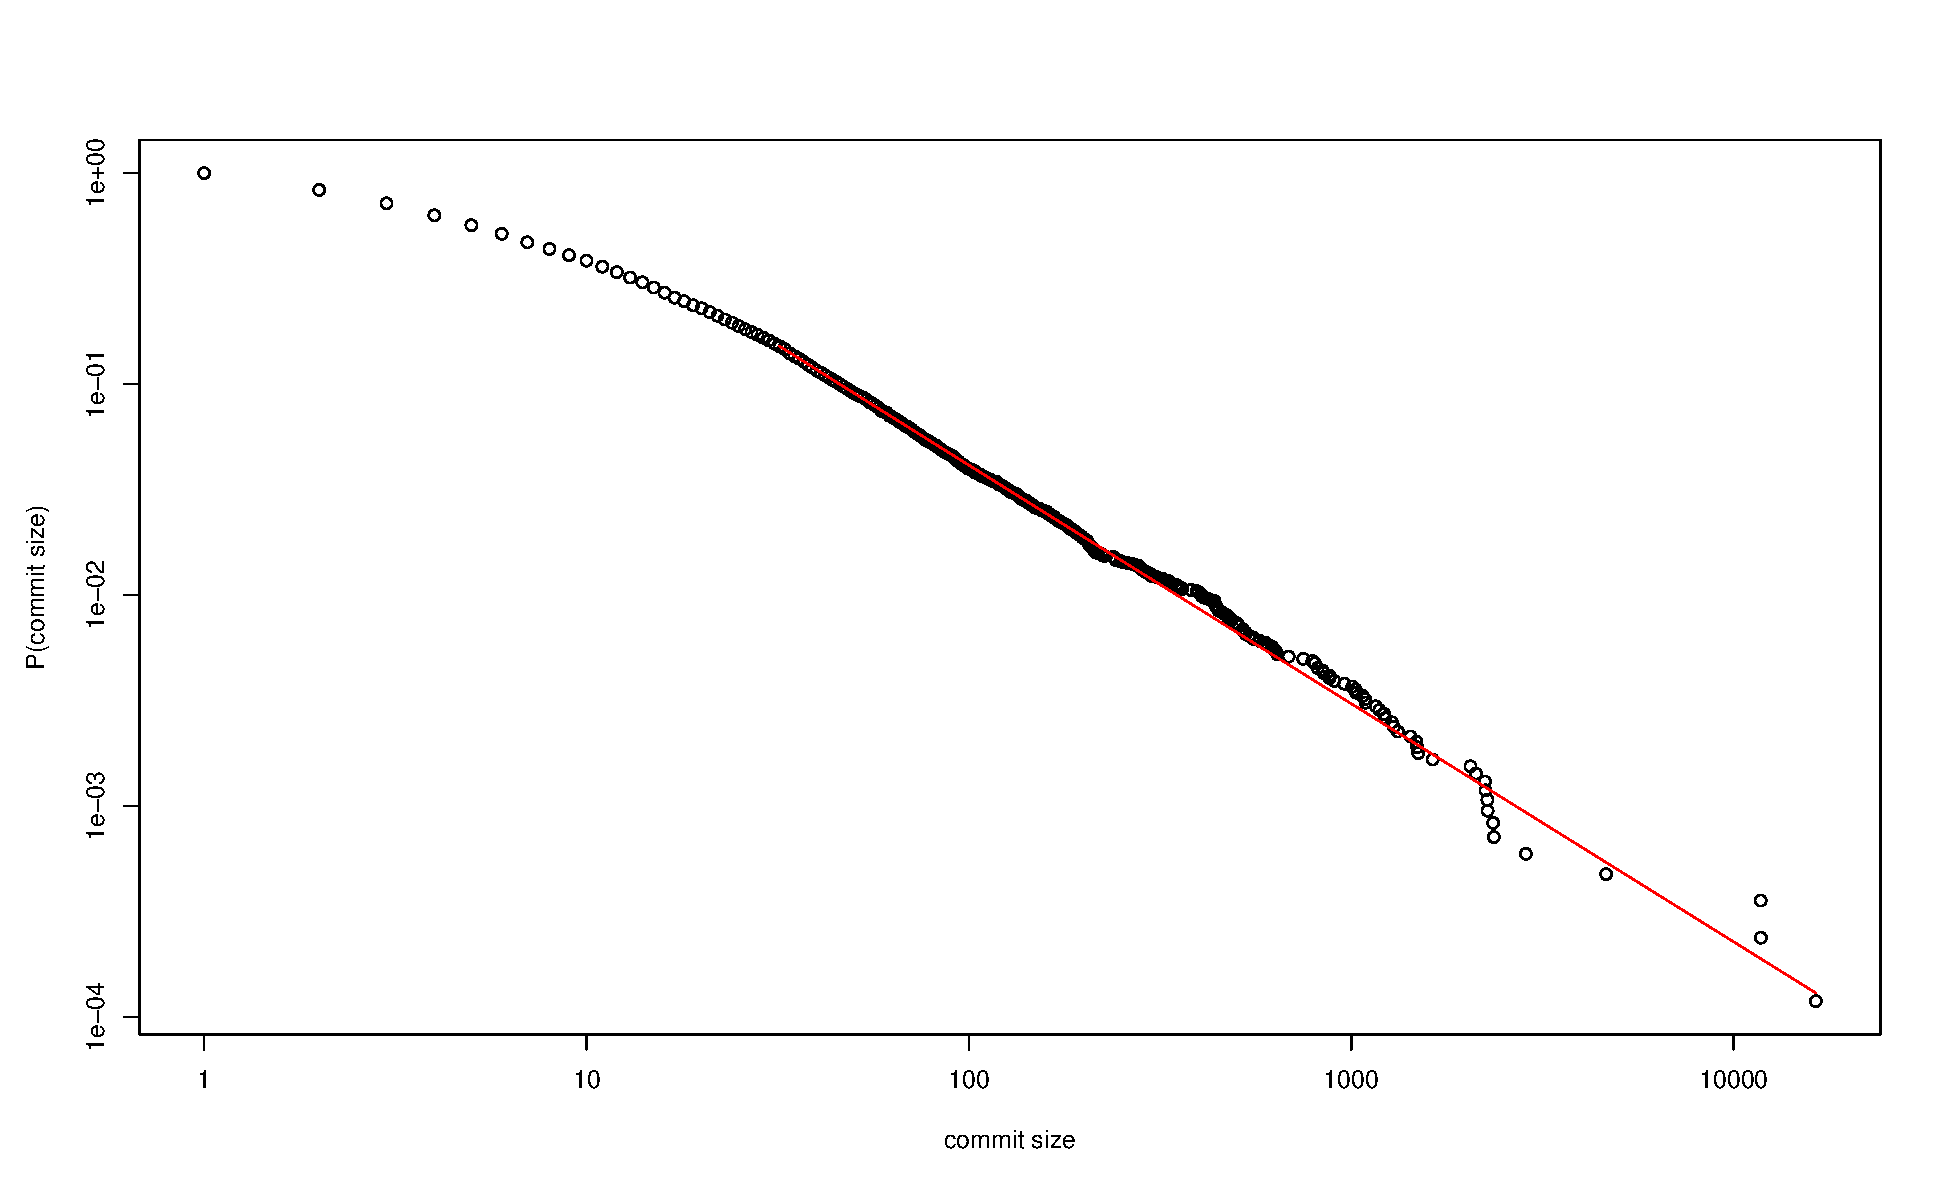
\includegraphics[width=0.95\textwidth]{plots/mojo-2017.eps}}
	\caption{PDF plot of a repository with \textit{Moderate} rank: Mojo from 2017.}
	\label{fig:mojo}
\end{figure*}



\begin{figure*}[htbp]
	\centerline{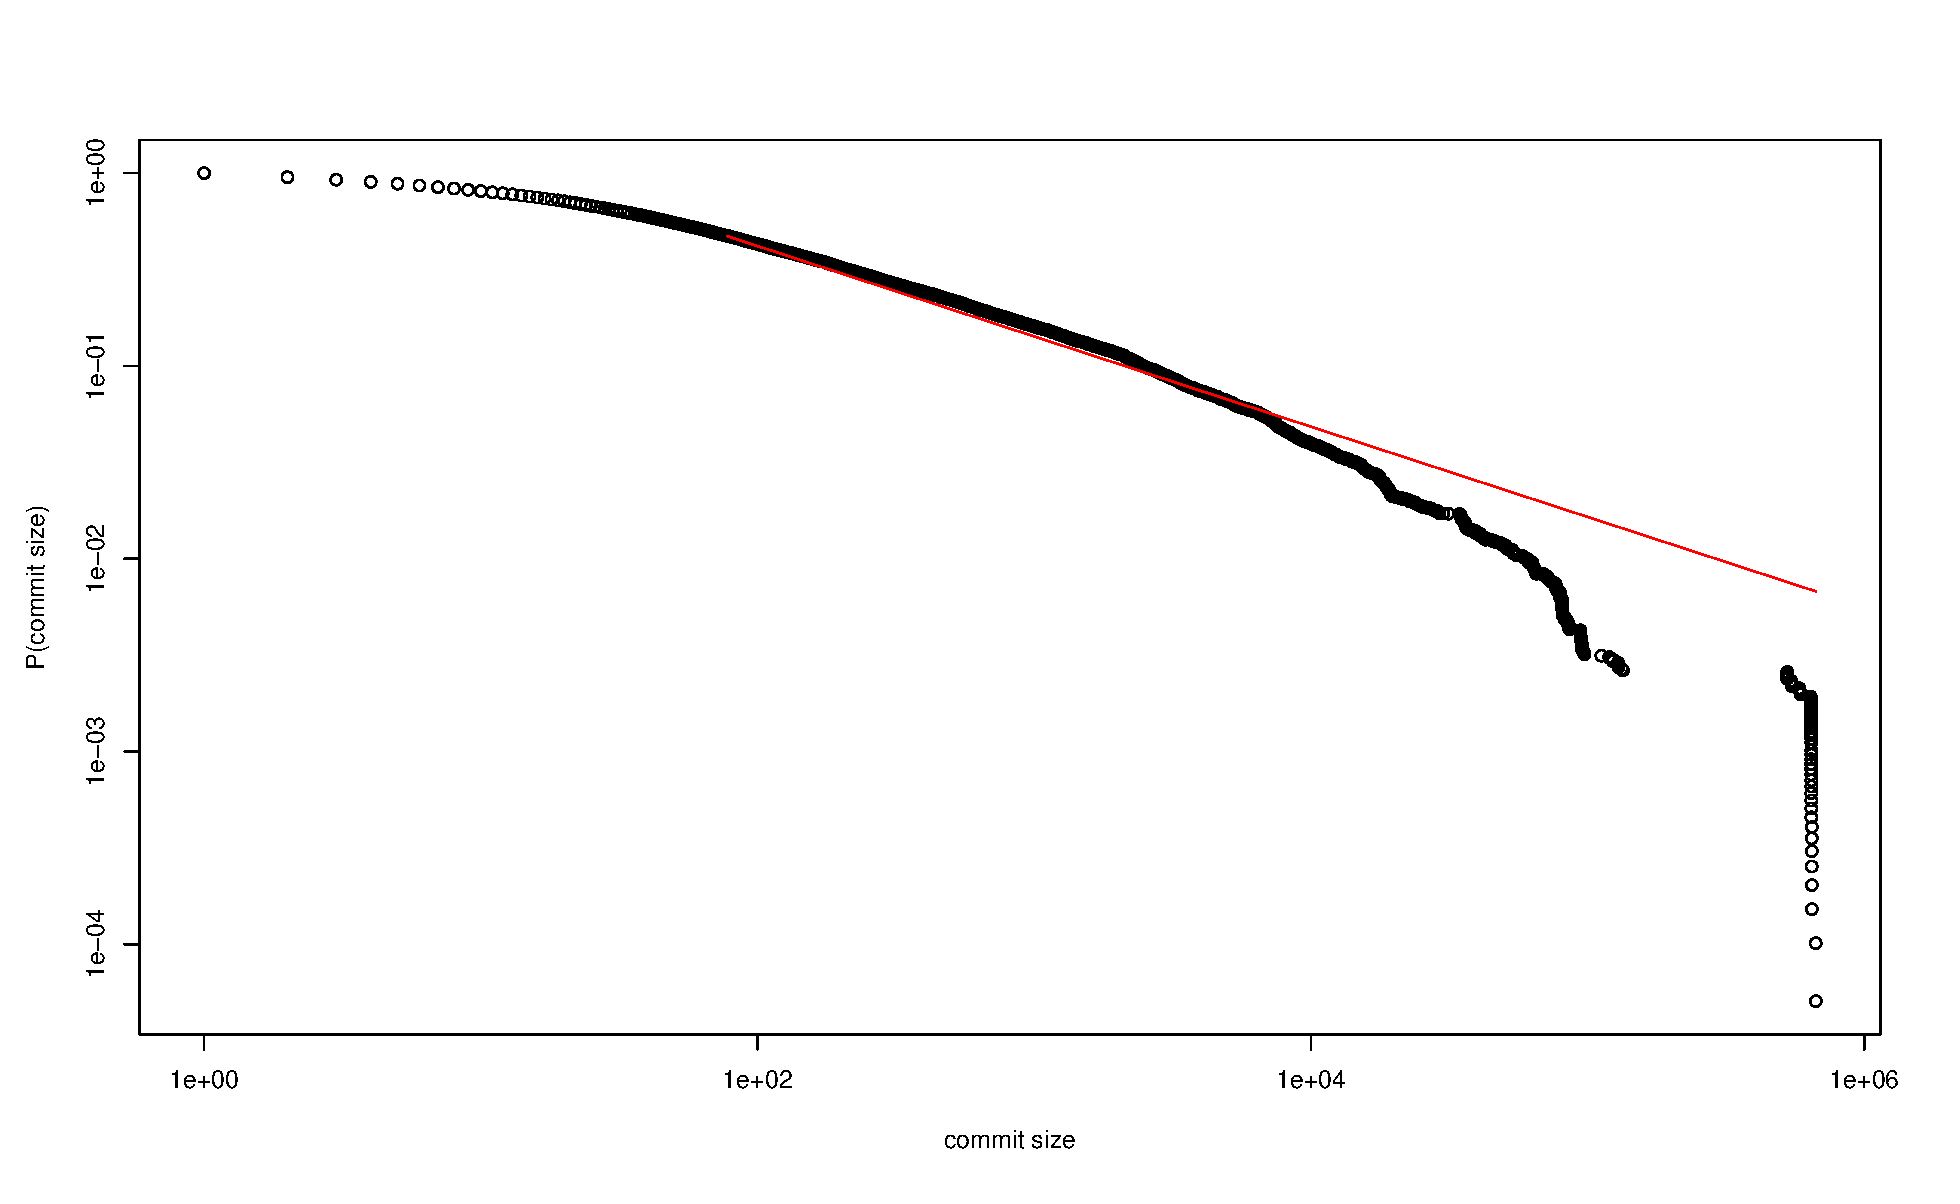
\includegraphics[width=0.95\textwidth]{plots/docker.eps}}
	\caption{PDF plot of a repository with \textit{None} rank: Docker from 2017.}
	\label{fig:docker}
\end{figure*}


% --------------------------------------------------------


\section{Conclusions}\label{conc}


% Several things we can do in the conclusions
% * So, most repositories are _not_ actually self-organized because they do not follow a power law? Answer: We can't affirm that. Power laws only manifest themselves in critical states; self-organization will still take place. 

In conclusion, there is still much to research in the evolution of software through code repositories.  %That's not a very good conclusion... That should be the conclusion to the conclusion - JJ

In general, the probability of finding a power law is quite low, so that up to now, and in the repositories studied, we can not affirm categorically that the system is in a critical state due to self-organization.

This result, however, does not imply that there is not any kind of self-organization or even a powerlaw, but that the system has not been regulated enough and, therefore has not been established near a possible critical state.

% Figures should be referenced in the results section, not the conclusions. - JJ
Faced with the most common visualizations, the one used in our paper highlights even more how we can not affirm the existence of power laws distributions. See as an example how Fig. \ref{fig:docker}. shows that the adjustment of a power law would not capture some characteristics in the tail of our data. 

On the other hand, Fig. \ref{fig:mojo}. is an example of when we can suspect the existence of a power law in the repository. A distribution that also remains in time till 2019. This can be an indicative that this repository is self-organizing to stay in that point.

Furthermore we would like to explore the possible causes of such dramatic changes as the ones seen in repositories like django and tensorflow, since they can be related to a possible phase change.

In any case, the article presents an adequate and objective workflow to study the existence of power law distributions that settles the status of these kind of measures in software development via repositories.

Thanks to this procedure, we hope we can constitute a new state of art, from which researchers can begin to study these and other properties of code repositories in order to understand which of them may be related to self-organization and which ones have a very low probability of that.  

% There is always a "future work" paragraph here. Where do you go from here?  - JJ


\bibliographystyle{apalike}
\bibliography{geneura,biblio}

\end{document}
